\documentclass{article}
\usepackage{graphicx}
\title{A proposal for the development of the networking device  for implementation of  private 5G networks}
\author{D. Manjunath, Madhav Desai,  L. Somappa, Gaurav Kasbekar\\ IIT Bombay\\ Abhijit Chaudhary \\ Niral Networks \\ Reapan Tikoo \\ Powai Labs}
\begin{document}
\maketitle

\section{Aims and Objective of the Project}

	The aim of the project is to build a trusted hardware platform
	which can be configured to form the core of a private 5G network.

	Networked devices, and devices that connect to other computing devices are 
	vulnerable to tampering and malicious compromise through both their software and hardware. 

	In our proposal, we will build a trusted hardware platform around 
	a core technology of the AJIT multi-threaded multi-core processor.   
	This processor has been developed at IIT Bombay, and has been used 
	successfully in the implementation of an IRNSS + GPS
	base-band receiver system.   Innovations such as route caching and packet
	flow interpreters will be integrated into the fabric of the proposed hardware
	platform.

	Further, the trusted hardware will run software which is completely open
	to user inspection and oversight.   The software is based on open source
	computations and will be ported to the hardware platform.

	The project will be executed under the supervision of IIT Bombay, 
	with contributions from IIT Bombay, Niral Networks, and Powai Lab
	Technologies Pvt. Ltd.


\section{Novelty of the proposed project}

	The novelty of the project can be summarized in four ways: trust,
	indigenous-ness, open software, scalability.
	
	\begin{itemize}
	\item Trust:
		The key elements in establishing trust are: 
		\begin{itemize}
			\item the identity of the developer institution and personnel, in this case led
			by IIT-Bombay.

			\item the transparency and documentation of the technology.
		\end{itemize}
	\item Made in India:
		Implies control over technology, longevity of the technology,
		cost advantages, independence and spin-offs.

	\item Non-proprietary software:
		Completely auditable, based on open standards, and with source
		code completely visible and shared.

	\item Scalability:
		The number of processor cores can be scaled to 64 and higher
		by introducing clustering of processor cores, and with a
		custom on-chip processor-NIC-memory network.
	\end{itemize}

	With this background, we propose a program of developing and deploying  private 5G subsystems.
	Our target deployment is the critical national infrastructure such as military establishments, 
	power grids, refineries, railways, shipyards, ordnance and armament factories, etc. 

	The hardware for such systems will be based on the work at IIT Bombay. The software will be from 
	Niral Networks who have been developing software-based communication systems.


\section{Detailed Description of the project: hardware platform}

	The project involves the development of a hardware network router using the
	AJIT multi-threaded multi-core processor, and the porting and customization of
	software from Niral Networks on to this router. 

	The hardware network router will be built using a multi-threaded multi-core
	64-bit AJIT processor, with four cores and eight threads.  The hardware
	router will be constructed in three phases over an 18 month period.

\subsection{Phase 1}

	In phase 1, a basic router which integrates the multi-core processor with
	four network interfaces will be built (See Figure \ref{fig:Phase1}):

\begin{figure}
  \centering
  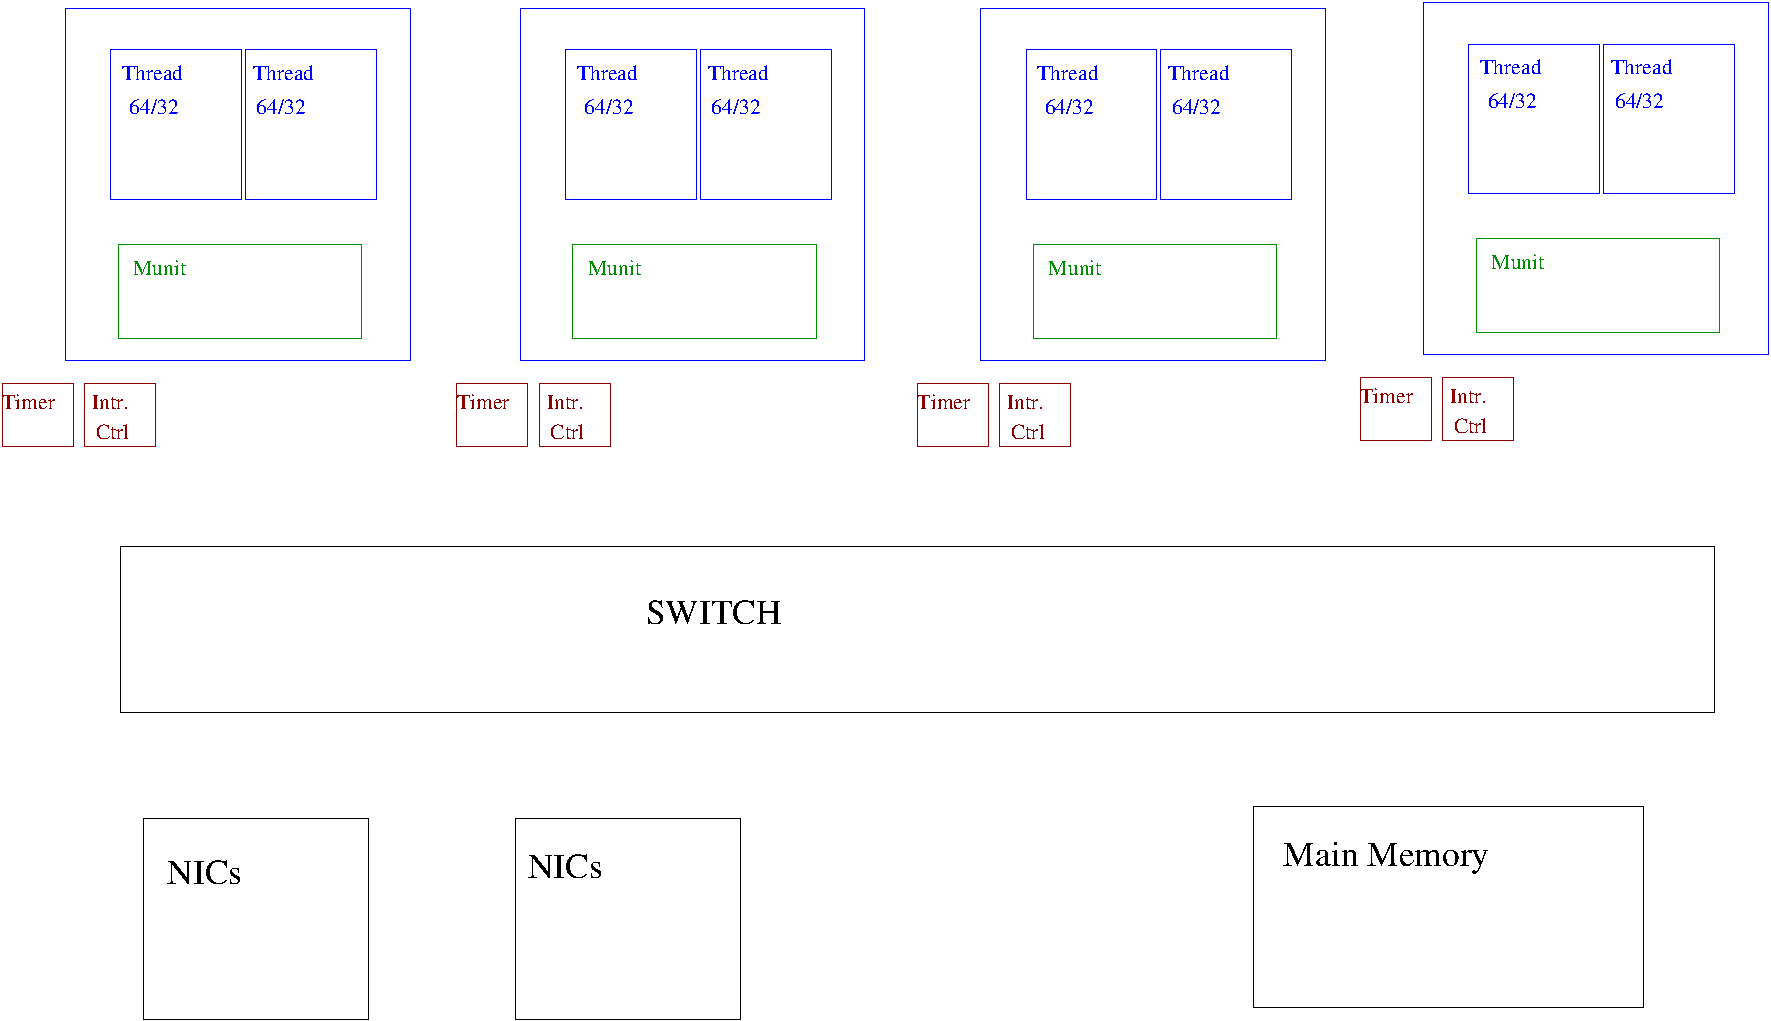
\includegraphics[width=12cm]{figs/Router_I.pdf}
  \caption{Router platform: phase 1}
  \label{fig:Phase1}
\end{figure}

The features of this platform are as follows:
\begin{itemize}
\item Vanilla NICs.
\begin{itemize}
\item NIC and main memory communicate directly.
\item NIC to NIC direct paths are provided.
\end{itemize}
\item Processor cores handle route lookup.
\item Software optimization.
\end{itemize}

\subsection{Phase 2}

\begin{figure}
  \centering
  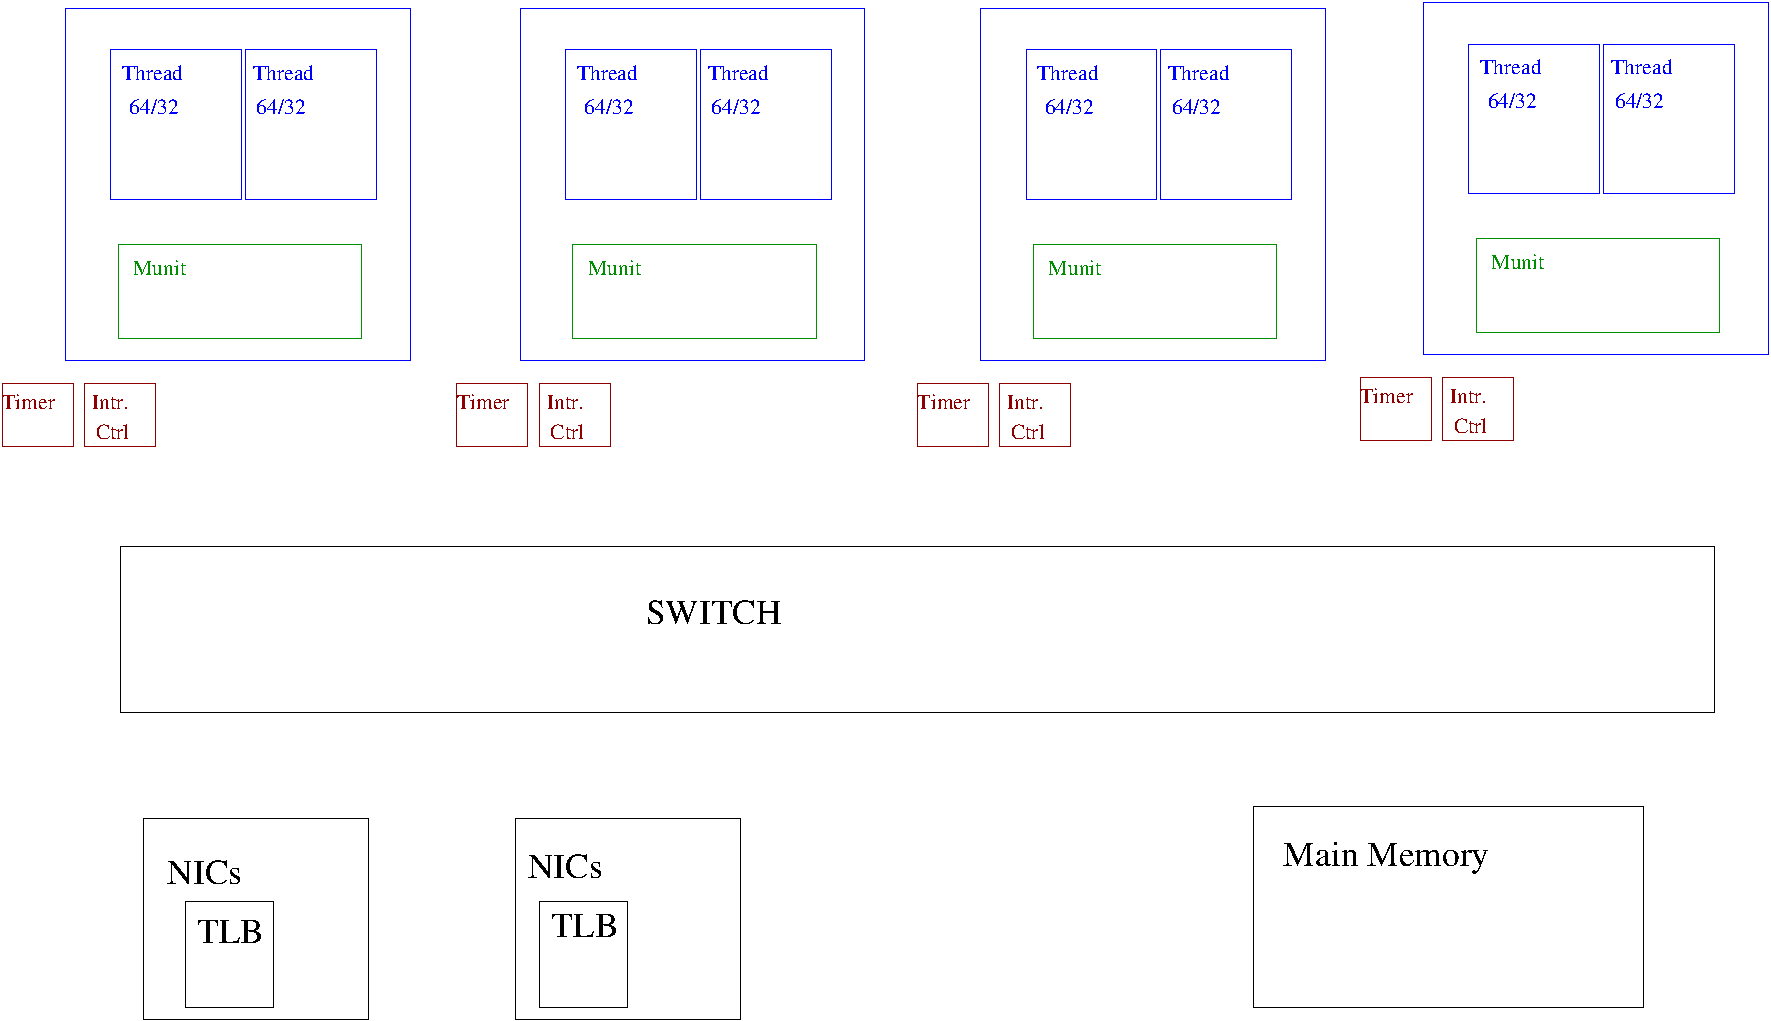
\includegraphics[width=12cm]{figs/Router_II.pdf}
  \caption{Router platform: phase 2}
  \label{fig:Phase2}
\end{figure}

In phase 2 (see Figure \ref{fig:Phase2}, 
the router will be enhanced with the following features:
\begin{itemize}
\item NICs with lookup caches.
\begin{itemize}
\item NIC and main memory communicate directly.
\item NIC to NIC communication is possible using
common switch.
\item On lookup cache hit, NIC to NIC packet
movement.
\item Packet modification in NIC.
\end{itemize}
\item Processor cores handle non-hit route lookups.
\end{itemize}
These enhancements aim at a 5X improvement over the Phase 1 router.

\subsection{Phase 3}
\begin{figure}
  \centering
  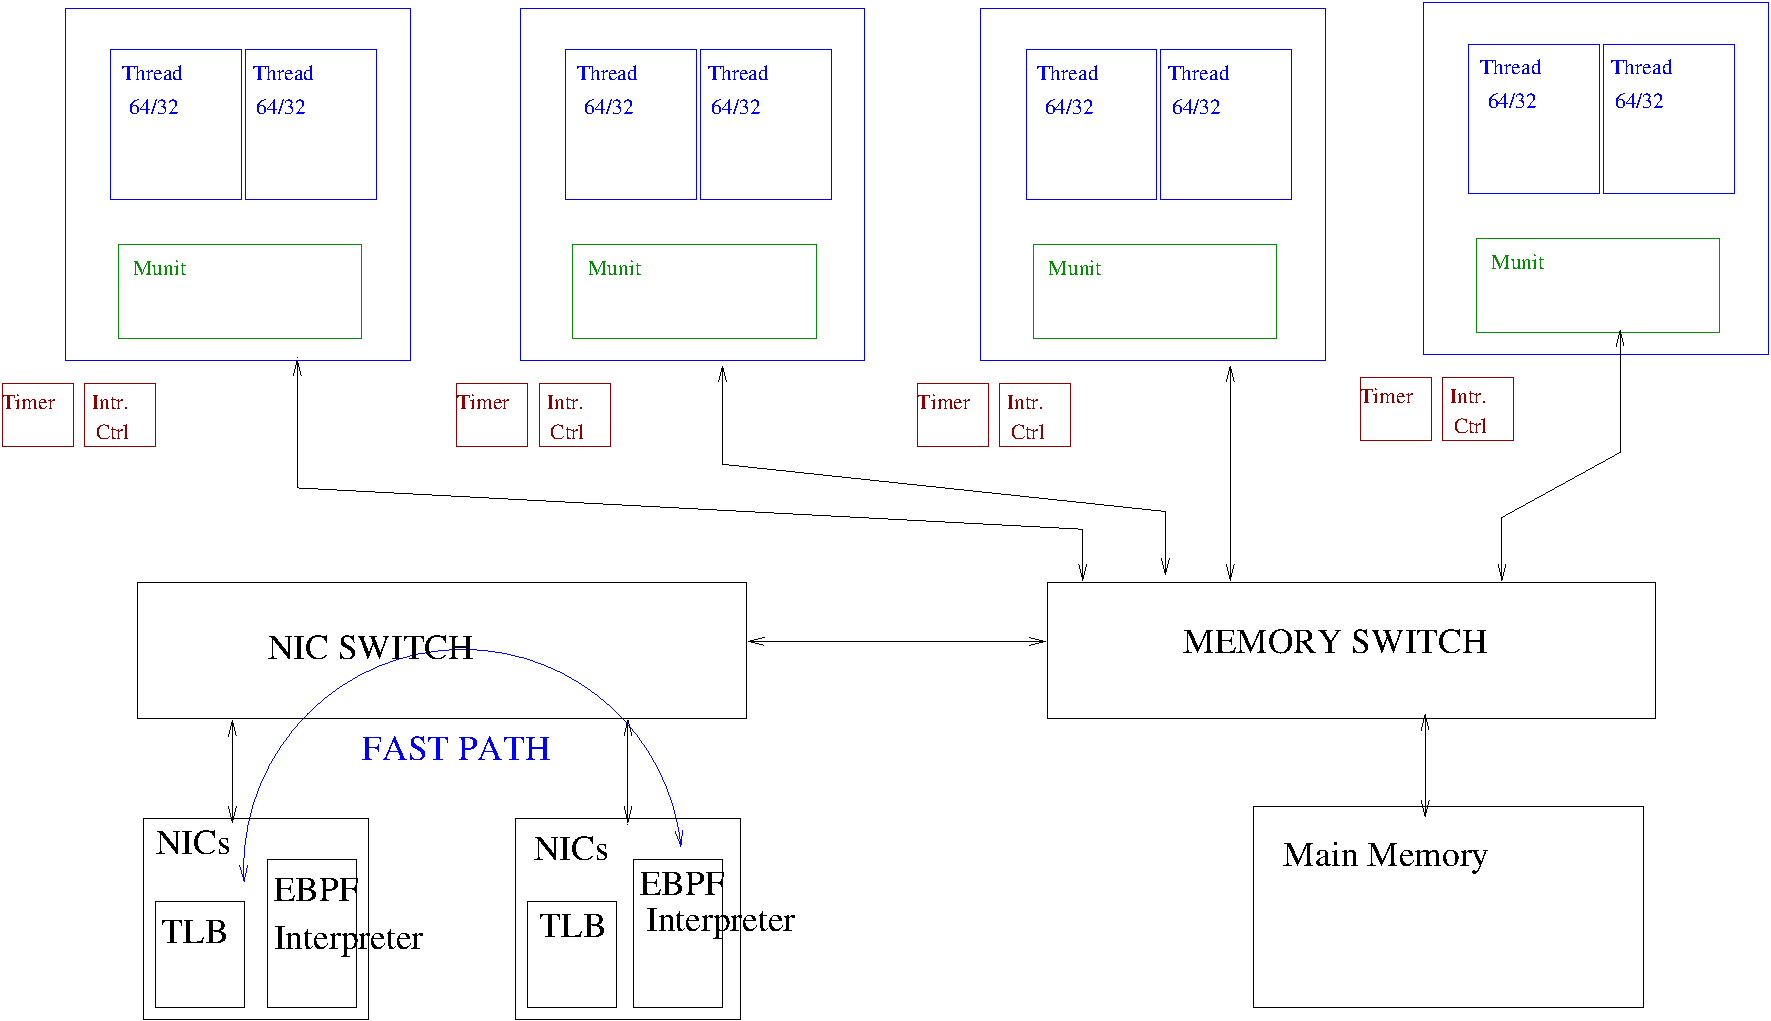
\includegraphics[width=12cm]{figs/Router_III.pdf}
  \caption{Router platform: phase 3}
   \label{fig:Phase3}
\end{figure}

In the phase 3 router, further enhancements will be
incorporated into the router platform.
\begin{itemize}
\item NICs with lookup caches and embedded EBPF interpreter.
\begin{itemize}
\item NIC and main memory communicate directly.
\item NIC to NIC high performance direct paths are provided via
separate switch.
\item Packet processing in NIC using EBPF interpreter.
\item On lookup cache or interpreter hit, NIC to NIC packet
movement.
\end{itemize}
\item Processor cores handle remaining route lookups.
\end{itemize}
As a result of these enhancements, we target a 5X performance
improvement over the Phase 2 router.

\subsection{Development process}

\begin{itemize}
\item Phase 1 (6 months):  port forwarding engine to 4-core 8-thread platform with vanilla NICs.
\item Phase 2 (6 months):  Control plane software port, add TLBs to NICs.
\item Phase 3 (6 months):  MPLS software port, add BPF interpreter to NICs.
\item On FPGA platform, demonstrate 1.6Gbps on Stage 1, 8 Gbps on Stage 2, 16 Gbps on Stage 3.
\item After FPGA validation, implement router ASIC (22nm, 1.2GHz, 10W).  Implementation will take 6-9 months.
\begin{itemize}
\item Target 100-200 Gbps in ASIC based router.
\end{itemize}
\end{itemize}

\section{Detailed Description of the project: software platform}

The software platform will support Layer-2 and Layer-3 features, with support for
\begin{itemize}
\item Layer-2 Processing including Ethernet, VLAN and ARP.
\item IPv4/IPv6 Packet Forwarding and Route Lookup.
\item MPLS/L3-VPN Forwarding and Label Management.
\item Centralized control plane to configure the IP routes or MPLS labels.
\end{itemize}

The software platform will be developed in three phases.

\subsection{Phase 1}

Development of the Layer 2, IPv4 and IPv6 forwarding stack and its integration to the AJIT Hardware. 

\subsection{Phase 2}

Development of the MPLS and L3-VPN forwarding stack and its integration to the AJIT Hardware.

\subsection{Phase 3}

Development of the Centralized Controller to remotely configure static IP routes or MPLS labels 
in the AJIT Hardware.

\section{Prototype deployment, validation and ASIC design}

A prototype router platform for use in private 5G networks will be deployed on the FPGA platform of 
the hardware outlined above. IPv4/IPv6 packet processing will be deployed as
part of phase 1, MPLS/L3-VPN will be deployed as part of Phase 2 and remote control plane 
configuration as part of Phase 3.  Concurrently engagement with potential end-users
(RailNet, Jio) will be initiated in order to identify a test-bed for prototype validation.

The ASIC design will be initiated at the end of the prototype validation phase.   The
target technology is currently 22nm UMC/TSMC, with a target core frequency of 1.2GHz.



\section{Responsibilities of the three institutions}

The participating institutions will have the following
responsibilities:
\begin{itemize}
\item IIT Bombay:  hardware design and validation, porting of software, ASIC design.
\item Niral Networks:  software development, customization, optimization, integration.
\item Powai Labs:  Management of ASIC production, system integration and validation with
potential end users.
\end{itemize}

\end{document}


